\documentclass[aspectratio=169]{../latex_main/tntbeamer}  % you can pass all options of the beamer class, e.g., 'handout' or 'aspectratio=43'
\usepackage{dsfont}
\usepackage{bm}
\usepackage[english]{babel}
\usepackage[T1]{fontenc}
%\usepackage[utf8]{inputenc}
\usepackage{graphicx}
\graphicspath{ {./figures/} }
\usepackage{algorithm}
\usepackage[ruled,vlined,algo2e,linesnumbered]{algorithm2e}
\usepackage{hyperref}
\usepackage{booktabs}
\usepackage{mathtools}

\usepackage{amsmath,amssymb}

\DeclareMathOperator*{\argmax}{arg\,max}
\DeclareMathOperator*{\argmin}{arg\,min}

\usepackage{pgfplots}
\pgfplotsset{compat=1.16}
\usepackage{tikz}
\usetikzlibrary{trees} 
\usetikzlibrary{shapes.geometric}
\usetikzlibrary{positioning,shapes,shadows,arrows,calc,mindmap}
\usetikzlibrary{positioning,fadings,through}
\usetikzlibrary{decorations.pathreplacing}
\usetikzlibrary{intersections}
\pgfdeclarelayer{background}
\pgfdeclarelayer{foreground}
\pgfsetlayers{background,main,foreground}
\tikzstyle{activity}=[rectangle, draw=black, rounded corners, text centered, text width=8em]
\tikzstyle{data}=[rectangle, draw=black, text centered, text width=8em]
\tikzstyle{myarrow}=[->, thick, draw=black]

% Define the layers to draw the diagram
\pgfdeclarelayer{background}
\pgfdeclarelayer{foreground}
\pgfsetlayers{background,main,foreground}

% Requires XeLaTeX or LuaLaTeX
\usepackage{unicode-math}

\usepackage{fontspec}
%\setsansfont{Arial}
\setsansfont{RotisSansSerifStd}[ 
Path=../latex_main/fonts/,
Extension = .otf,
UprightFont = *-Regular,  % or *-Light
BoldFont = *-ExtraBold,  % or *-Bold
ItalicFont = *-Italic
]
\setmonofont{Cascadia Mono}[
Scale=0.8
]

% scale factor adapted; mathrm font added (Benjamin Spitschan @TNT, 2021-06-01)
%\setmathfont[Scale=1.05]{Libertinus Math}
%\setmathrm[Scale=1.05]{Libertinus Math}

% other available math fonts are (not exhaustive)
% Latin Modern Math
% XITS Math
% Libertinus Math
% Asana Math
% Fira Math
% TeX Gyre Pagella Math
% TeX Gyre Bonum Math
% TeX Gyre Schola Math
% TeX Gyre Termes Math

% Literature References
\newcommand{\lit}[2]{\href{#2}{\footnotesize\color{black!60}[#1]}}

%%% Beamer Customization
%----------------------------------------------------------------------
% (Don't) Show sections in frame header. Options: 'sections', 'sections light', empty
\setbeamertemplate{headline}{empty}

% Add header logo for normal frames
\setheaderimage{
	% 
\includegraphics[height=\logoheight]{figures/TNT_darkv4.pdf}
	
\includegraphics[height=\logoheight]{../latex_main/figures/luh_logo_rgb_0_80_155.pdf}
	% 
\includegraphics[height=\logoheight]{figures/logo_tntluh.pdf}
}

% Header logo for title page
\settitleheaderimage{
	% 
\includegraphics[height=\logoheight]{figures/TNT_darkv4.pdf}
	
\includegraphics[height=\logoheight]{../latex_main/figures/luh_logo_rgb_0_80_155.pdf}
	% 
\includegraphics[height=\logoheight]{figures/logo_tntluh.pdf}
}

% Title page: tntdefault 
\setbeamertemplate{title page}[tntdefault]  % or luhstyle
% Add optional title image here
%\addtitlepageimagedefault{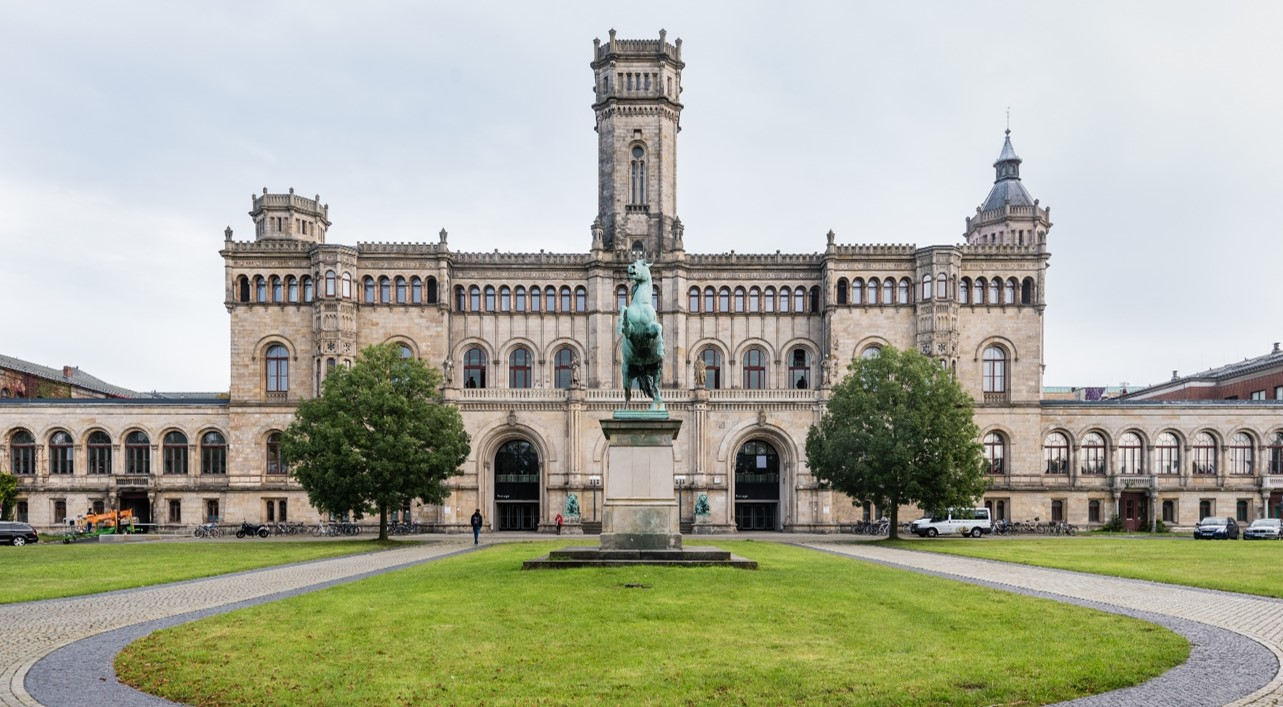
\includegraphics[width=0.65\textwidth]{figures/luh_default_presentation_title_image.jpg}}

% Title page: luhstyle
% \setbeamertemplate{title page}[luhstyle]
% % Add optional title image here
% \addtitlepageimage{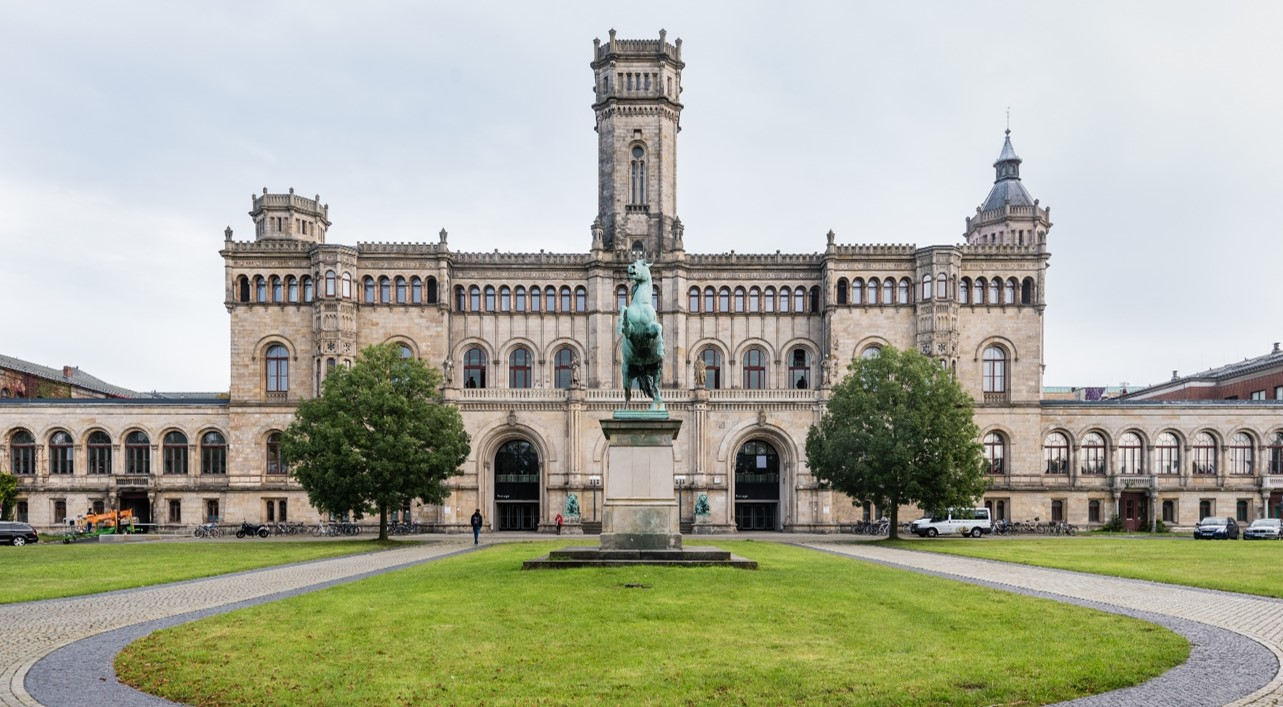
\includegraphics[width=0.75\textwidth]{figures/luh_default_presentation_title_image.jpg}}

\author[Lindauer \& Anand]{Marius Lindauer and Avishek Anand\\[1em]
	
\includegraphics[height=\logoheight]{../latex_main/figures/luh_logo_rgb_0_80_155.pdf}\qquad

\includegraphics[height=\logoheight]{../latex_main/figures/TNT_darkv4}\qquad

\includegraphics[height=\logoheight]{../latex_main/figures/L3S.jpg}	}
\date{Winter Term 2021
}


%%% Custom Packages
%----------------------------------------------------------------------
% Create dummy content
\usepackage{blindtext}

% Adds a frame with the current page layout. Just call \layout inside of a frame.
\usepackage{layout}


\title[Introduction]{iML: Local Explanations}
\subtitle{Counterfactuals}

%\institute{}


\begin{document}
	
	\maketitle

	%-----------------------------------------------------------------------------------------------------------------------------


\begin{frame}{Counterfactual Explanations}
	\begin{itemize}
	    \item \alert{Counterfactual explanations} (CEs) or short \alert{counterfactuals} explain particular decisions of an ML model by presenting an alternative input whose prediction equals a desired outcome.
	    \smallskip \pause
		\item CEs represent \alert{close neighbors} of a data point we are interested in,\\ but belonging to the \alert{desired outcome class}. 
		\smallskip \pause
		\item[$\leadsto$] CEs reveal what minimal changes to the input are sufficient to receive a different response.
		\begin{itemize}
		    \item Very useful if there is a chance to change the input futures (e.g., by changing behaviour)
		\end{itemize}
		\smallskip \pause
		\item Due to their natural interpretation, the targeted audience of CEs are often end-users not ML engineers.
%		\item While we focus here exclusively on their application to tabular data, they can also be applied to image and text data. 
	\end{itemize}
\end{frame}

\begin{frame}{Example: Credit Risk Application} 
	\begin{itemize}
		\item $x$: customer and credit information
		\item $y$: grant or reject credit
	\end{itemize}
	\begin{center}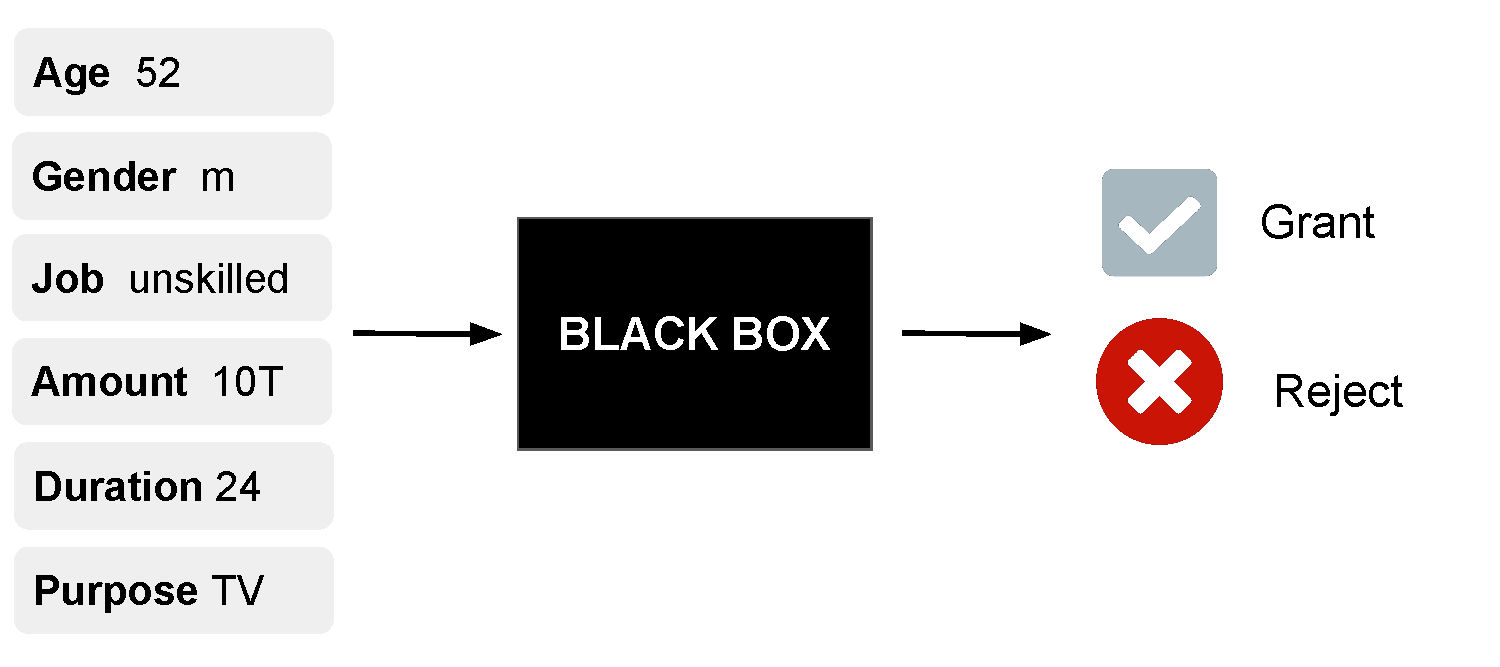
\includegraphics[width=0.4\linewidth, page=1]{figure/counterfactuals_credit.pdf} \end{center}
	
	Questions: 
	\begin{itemize}
		\item Why was the credit rejected? 
		\item Is it a fair decision? 
		\item How should $x$ be changed so that the credit is accepted?  
	\end{itemize}
	
	\end{frame}
	%-------------------------------------------
	\begin{frame}{Example: Credit Risk Application} 
	
	Counterfactual Explanations provide answers in the form of "What-If"-scenarios. 
	\begin{center}\includegraphics[width=0.4\linewidth, page=2]{figure/counterfactuals_credit.pdf} \end{center}
	
	``If the person was more skilled and the credit amount had been reduced to \$8.000, his credit would have been granted."  \\[0.2cm]
	
\end{frame}

\begin{frame}{Aims \& Roles}
	CEs can serve various purposes, the user can decide what to learn from them. For example:\newline
	``If the person had been one year older and the credit amount had been increased to \$12.000, her credit would have been granted."  \\[0.2cm]
	\begin{itemize}
		\itemsep1.3em
		\pause
		\item \textbf{Guidance for future actions:} \textit{Ok, I'll apply again next year for the higher amount.}
		\pause
		\item \textbf{Provide reasons:} \textit{Interesting, I did not know that age plays a role in loan applications.}
		\pause
		\item \textbf{Provide grounds to contest the decision:} \textit{How dare you, I do not want to be discriminated for my age in an application.}
		\pause
		\item \textbf{Detect model biases:} \textit{There is a bug, an increase in amount should not increase approval rates.}
	\end{itemize}
\end{frame}

% \begin{frame}{Philosophical Basis}
% Counterfactuals have a long-standing tradition in analytic philosophy.
% Accoding to Lewis (1973), a \textbf{counterfactual conditional} is a statement of the form:	
% \begin{equation}
% 		\textnormal{``If $S$ was the case, $Q$ would have been the case."}
% 		\label{eq:sent}
% \end{equation}
% 	\begin{itemize}
% 		\item $S$ must relate to a past event that didn't occur. In that sense counterfactuals run \textbf{contrary} to the \textbf{facts}.
% 		\item In Lewis's framework Statement~(\ref{eq:sent}) is true, if in all possible worlds most similar to the actual world where $S$ had been the case, $Q$ would have been the case. 
% 		\item A world is similar to another if laws are maximally preserved between the worlds and only a few facts are changed.
% 	\end{itemize}
% \end{frame}

% \begin{frame}{Philosophical Basis}
% 	\begin{itemize}
% 	\item Counterfactuals have largely been studied to give an account of causal dependence.
% 		\item Causal dependence underlies the explanatory power CEs offer. Good CEs point to the critical causal factors that drove the algorithmic decision.
% 		\item If maximal closeness is relaxed, causally irrelevant factors can become part of the explanation. Think of a case when a decrease in amount by \$20.000 and being one year older is recommended by the explainer to receive the loan while changing only the former suffices.
% 		\item CEs are often contrastive, i.e., they explain a decision by referring to an alternative outcome. E.g., if the loan-applicant was 30 instead of 60 years old, the approved loan would have been over \$100.000 instead of \$40.000.
% 	\end{itemize}
% \end{frame}


\begin{frame}{Mathematical Perspective \lit{Dandl et al. 2020}{https://arxiv.org/abs/2004.11165} \lit{Verma et al. 2020}{https://arxiv.org/pdf/2010.10596.pdf}}
	Terminology: 
	\begin{itemize}
		\item $x$ as original/factual datapoint whose prediction we want to explain
		\item $y' \subset \mathbb{R}^g$ as desired prediction ($y' = 1000$ or $y' = $``grant credit"). %It could be also an interval ($y' = [1000, \infty[$).
	\end{itemize}
	\vspace{0.3cm}
	A \textbf{valid} counterfactual $x'$ is a datapoint: 
	\begin{enumerate}
		\item whose prediction $\hat{f}(x')$ is equal to the desired prediction $y'$. 
		\item that is \alert{maximally close} to the original datapoint $x$.
	\end{enumerate}
	\pause
	As an optimization problem with two objectives: 
	\begin{equation}
		\argmin_{x'} o_1(\hat{f}(x'), y') + \lambda o_2(x', x).
		\label{eq:optim}
	\end{equation}
	
	
	\begin{itemize}
		\item $\lambda$ balances the two objectives.
		\item $o_1$ and $o_2$ are distance metrics on the prediction space and feature space, resp.
	 \end{itemize}
\end{frame}	 

% \begin{frame}{Mathematical Perspective \lit{Dandl et al. 2020}{https://arxiv.org/abs/2004.11165} \lit{Verma et al. 2020}{https://arxiv.org/pdf/2010.10596.pdf}}

%     \begin{itemize}		
% 		\item For regression, $o_1$ could be, e.g., the L1-distance $o_1(\hat{f}(x'), y') = |\hat{f}(x')-y'|$. \\For classification, L1-distance is suitable for scores and the indicator function $o_1(\hat{f}(x'), y') = \mathrm{I}_{\{ \hat{f}(x') \neq y' \}}$ for labels. 
% 		\item $o_2$ could be the Gower distance that is suitable for mixed features: 
% 		$$o_2(x', x) = \Gower(x', x) = \frac{1}{p}\sum_{j = 1}^{p} \delta_G(x'_j, x_j)	\in [0, 1]$$
% 		The value of $\delta_G$ depends on the feature type:
% 		\begin{equation*}
% 		\delta_G(x'_j, x_j) = 
% 		\begin{cases}
% 		\frac{1}{\widehat{R}_j}|x_j'- x_j| & \text{if $x_j$ is numerical} \\
% 		\Ind_{\{ x_j' \neq x_j \}} & \text{if $x_j$ is categorical}
% 		\end{cases}
% 		\end{equation*}
% 		with $\widehat{R}_j$ as the value range of feature $j$ in the training dataset. 
% 	\end{itemize}
% \end{frame}

\begin{frame}[c]{Further Objectives \lit{Verma et al. 2020}{https://arxiv.org/pdf/2010.10596.pdf}}
	
	\textbf{Sparsity:}
	\begin{itemize}
		\item End-users often prefer short over long explanations. For CEs this means that the changes made to obtain counterfactuals must be \textbf{sparse}. 
		\item The distance $o_2$ can but does not necessarily take the number of changed features into account. Prominent examples that do so are the L$_0$- and the L$_1$-norm.
        \item We can also account for sparsity by adding an extra term to our objective that counts the number of changed features via the L$_0$-norm $$o_3(x', x) = \sum_{j = 1}^p \mathrm{I}_{\{ x'_j \neq x_j \}}.$$ 
	\end{itemize}
	
\end{frame}
%----------------------------------------------------------------------------
\begin{frame}[c]{Further Objectives \lit{Verma et al. 2020}{https://arxiv.org/pdf/2010.10596.pdf}}
	
	\begin{columns}
	\begin{column}{0.55\textwidth}
		\textbf{Plausibility:}
		\begin{itemize}
			\item CEs should suggest alternatives that are plausible. E.g, it is a bad idea to suggest a loan applicant to raise her income and get unemployed at the same time. 
			\item Thus, we desire realistic CEs in the sense that they originate from the distribution of $\mathcal{X}$ or adhere to the data manifold. 
			\item Estimating a joint distribution over the training data is a complex, especially for mixed feature spaces. As a proxy, we could \alert{desire that $x'$ is close to the training data.}
		\end{itemize}	
	\end{column}
	\begin{column}{0.4\textwidth}
	
		\begin{center}
			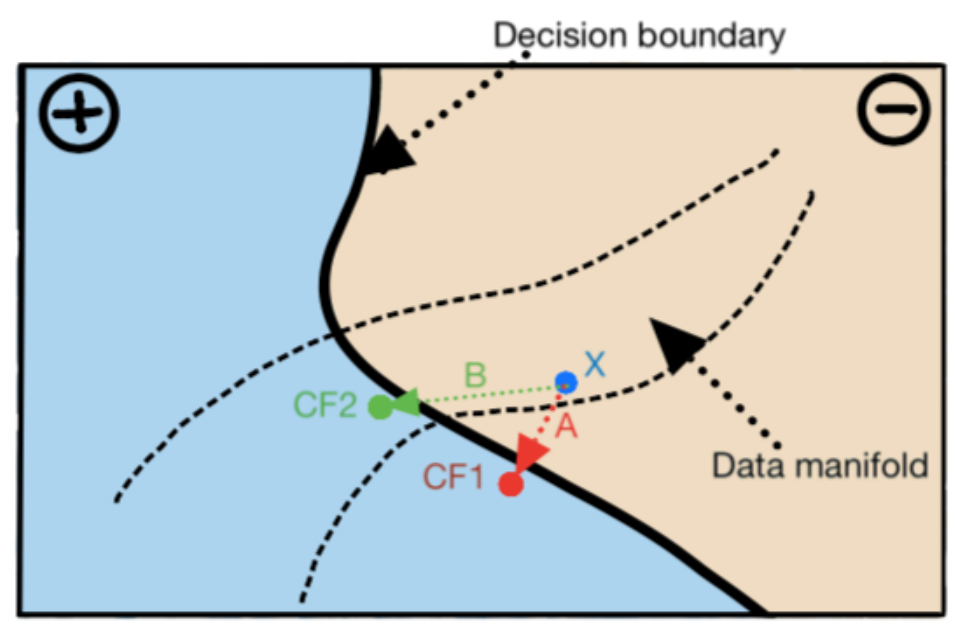
\includegraphics[width=1\textwidth]{figure/counterfactuals_obj}
		\end{center}
		
	    Source: \lit{Verma et al. 2020}{https://arxiv.org/pdf/2010.10596.pdf}
		
		\vspace{0.3cm}
	\end{column}
	\end{columns}

\end{frame}

\begin{frame}[c]{The Rashomon Effect}
	\begin{itemize}
	    \item Several equally good CEs are possible: \alert{Rashomon effect}
	    \pause\smallskip
		\item We could present all CEs for a given case; however, human processing capacity is limited.
		\pause\smallskip
		\item By which criterion should a few CEs be selected?
		\pause\smallskip
		\item As the model is generally non-linear, inconsistent CEs can arise, e.g. suggesting either an increase or decrease in credit duration.
		\pause\smallskip
		\item[$\leadsto$] Open problem in IML.
	\end{itemize}
\end{frame}

% \begin{frame}{Remarks: Model or Real-World \lit{Karimi et al. 2021}{https://arxiv.org/abs/2002.06278}}
% Most CEs provide explanations of model-predictions. However, to end-users, these explanations appear to explain the process in which the model is employed. Unfortunately, the transfer from the model to the real-world is generally not permitted.
% 	\begin{itemize}
% 	\item Consider, e.g., a CE that proposes to increase the feature age by 5 to obtain the loan. A loan applicant takes this information and applies 5 years later for the loan. 
% 	\item However, by then, many of her properties have changed not only the age since they are causally dependent on age like income or the job status.
% 	\item Karimi et al. (2020) avoid this shortcoming by considering causal dependencies between variables.
% 	\end{itemize}
% \end{frame}


%------------------------------------------------------------------------------------
%------------------------------------------------------------------------------------

\begin{frame}[c]{Overview of Methods}
	Multiple methods for calculating CEs. Differ greatly in: 
	\begin{itemize}
		\item \textbf{Targets:} Most methods focus on classification models, only few cover regression models. 
		\pause
		\item \textbf{Data Types:} Mainly for tabular data, few methods focus on visual/text data, none on audio.
		\pause
		\item \textbf{Feature space:} Some only handle numerical features, few process discrete and continuous. 
		\pause
		\item \textbf{Objectives:} Many methods focus on action guidance, plausibility and sparsity, few on other objectives like \alert{fairness or individual preferences}.
        \pause
		\item \textbf{Model access:} Both model-agnostic and model-specific methods exist.
		\pause
		\item \textbf{Optimization tool:} Gradient-based algorithms (only for differential models), mixed-integer programming (only linear) or gradient-free algorithms e.g. Nelder-Mead, genetic algorithm. 
		\pause
		\item \textbf{Rashomon Effect:} Many methods return a single counterfactual per run, some multiple counterfactuals, others prioritize CEs or let the user choose.
	\end{itemize}
\end{frame}

\begin{frame}[c]{Single-Objective Counterfactual Explanations \lit{Wachter et al. 2018}{https://arxiv.org/abs/1711.00399}}

	\begin{equation}
		\argmin_{x'} \max_{\lambda} \lambda \underbrace{(\hat{f}(x') - y')^2}_{o_1(\hat{f}(x'), y')} + \underbrace{\sum\nolimits_{j = 1}^p |x'_j - x_j|/\text{MAD}_j}_{o_2(x', x)}.
		\label{eq:wachter}
	\end{equation}
	
	$\text{MAD}_j$ is the median absolute deviation of feature $j$. In each iteration, optimisers like ADAM or Nelder-Mead solve Eq.~(\ref{eq:wachter}) for $x'$ and then $\lambda$ is increased until a sufficiently close solution is found. \\[0.2cm]
	
	This optimization problem has several shortcomings: 	
	\begin{itemize}
		\item We do not know how to choose $\lambda$ a priori. 
		\item Due to the maximization of $\lambda$ we focus primarily on the minimization of $o_1$.\\
		Only if $\hat{f}(x') = y'$, we focus on minimizing $o_2$. 
		\item The definition of $o_2$ only covers numerical features. 
		\item Sparsity and plausibility of counterfactuals are neglected. 
	\end{itemize}

\end{frame}

\begin{frame}{Multi-Objective Counterfactual Explanations \lit{Dandl et al. 2020}{https://arxiv.org/abs/2004.11165}}
	\begin{itemize}
		\item Instead of collapsing objectives into a single objective, we could optimize all four objectives simultaneously
	$$	\argmin_{x'} \left(o_1(\hat{f}(x'), y'), o_2(x', x), o_3(x', x), o_4(x', \Xmat) \right). $$
		
		\item Note that weighting parameters like $\lambda$ are not necessary anymore. 
		\item Adjusted by the multi-objective genetic algorithm (NSGA-II) to produce a set of diverse counterfactuals for mixed discrete and continuous feature spaces.
		\item Instead of one, the algorithm returns a set of counterfactuals that represents different trade-offs between the objectives and are constructed to be diverse in feature space.
	\end{itemize}
\end{frame}




%\begin{frame}{Example: Bike Sharing Dataset}
%	\begin{itemize}
%		\item Model: Random Forest with 500 trees
%		\item $x$ is the first data point of the dataset with $\hat{f}(x) = 1767.93$ rental bikes. 
%		\item Our desired goal is to increase the count of total rental bikes to $y' = [3000, \infty[$
%		\item MOC (with default parameters) found 56 counterfactuals after 200 iterations that met the target.
%		\item Most counterfactuals proposed to decrease the humidity (94.6 \%) and more than half to increase the temperature (55.4\%). 
%		\item Some counterfactuals proposed additional changes to the year (2012 instead of 2011) and month (December instead of Januar).
%		\framebreak 
%		\item We can visualize feature changes with a parallel plot. 
%		\item For humidity and temperature, we can additionally show a 2-dim surface plot. 
%	\end{itemize}
%	\vspace{-0.5cm}
%	\begin{columns}
%		\begin{column}{0.5\textwidth}
%			\begin{center}
%				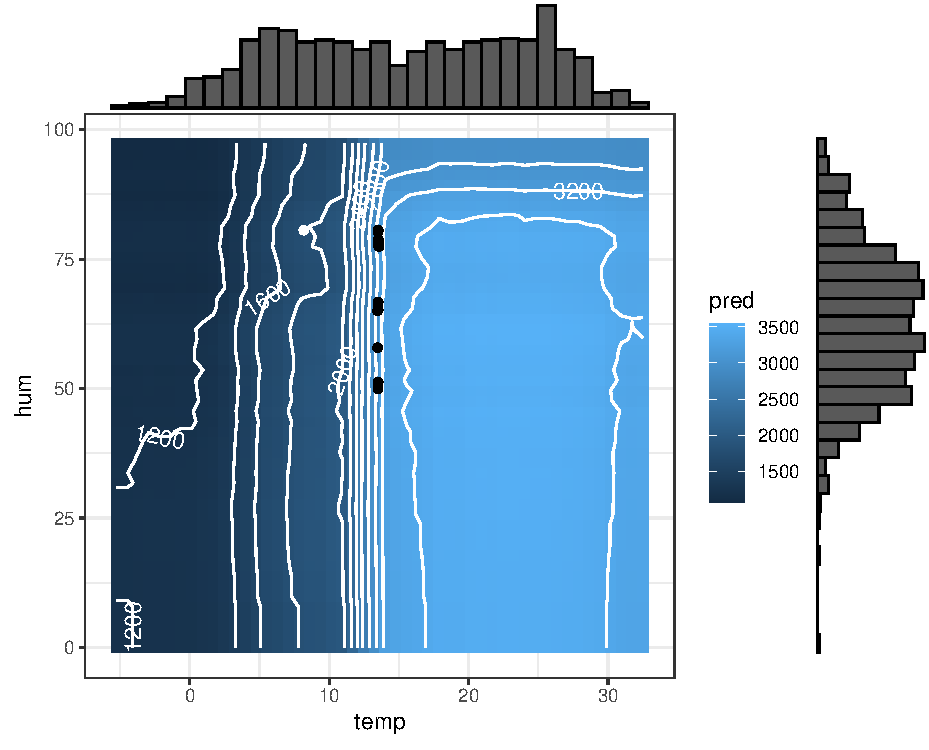
\includegraphics[width=1\textwidth]{figure/counterfactuals_bike_sp}
%			\end{center}
%		
%			\scriptsize{\textbf{Figure:} Response surface plot. 
%				The white dot is $x$, black dots are $x'$. The histograms display the marginal distribution of the training data $\Xmat$.} 
%				
%		\end{column}
%		\begin{column}{0.5\textwidth}  
%			\begin{center}
%				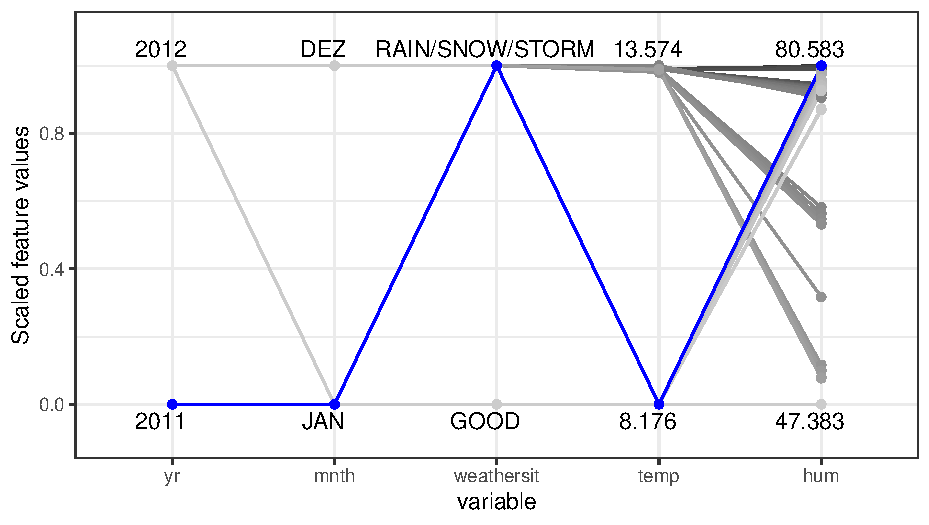
\includegraphics[width=1\textwidth]{figure/counterfactuals_bike_para}
%			\end{center}
%		
%		\scriptsize{\textbf{Figure:} Parallel plot. 
%			The grey lines show the feature values of the counterfactuals $x'$, the blue line corresponds to the values of $x$. Features without proposed changes are omitted. The bold numbers give minima and minima of numeric features while character strings indicate categories of character features.} 
%		
%		\end{column}
%	\end{columns}
%\end{frame}



\end{document}